\chapter{Direccionamiento IPv4}

La \textbf{dirección IP} es el identificador (que debe ser único) de un dispositivo dentro de una red. Los dispositivos pertenecientes a la misma red podrán comunicarse entre sí mediante dicha dirección IP. Todas las características que conforman esta IP están explicados en el \textbf{protocolo IP} (\href{https://es.wikipedia.org/wiki/Protocolo_de_internet}{Internet Protocol}).

Debido a que en el origen de la creación del protocolo IPv4 no se pensaba que llegase a haber tantos dispositivos conectados a internet, el límite que se puso para el número de posibles direcciones está llegando a su fin. Es por ello que ya existe un nuevo protocolo, \textbf{IPv6} desde hace tiempo, que sustituirá a IPv4 en un futuro, pero para ello debe de realizarse una transición que no termina de finalizar, aunque ya es posible hacer uso de ello.

El direccionamiento IP proporciona un mecanismo para la asignación de identificadores a cada dispositivo conectado a una red. Antes de dar información más técnica, exponemos los principales conceptos:

\begin{itemize}
    \item Una dirección IP es un conjunto de bits (que formarán 4 números decimales), que sirve para identificar de forma única a un dispositivo dentro de la red.
    \item La asignación de dicha IP se puede realizar de dos maneras:
    \begin{itemize}
        \item \textbf{Estática}: El administrador del dispositivo deberá configurar la dirección de manera manual teniendo en cuenta los parámetros necesarios que se ajusten a la red a la que se quiere conectar.
        \item \textbf{Dinámica}: Una vez el dispositivo se conecte de manera física a la red (por cable, o en caso de ser de manera inalámbrica, realizando la conexión  al SSID e introduciendo la contraseña) habrá un servicio (\textbf{DHCP}) que le otorgará una IP.
    \end{itemize}
\end{itemize}

El protocolo IPv4 permite la existencia de dos tipos de direcciones:

\begin{itemize}
    \item \textbf{Direcciones públicas}: Son las utilizadas en Internet. Cualquier dispositivo que se conecte de manera directa a Internet debe tener un direccionamiento público. Existe la organización \href{https://es.wikipedia.org/wiki/Corporaci%C3%B3n_de_Internet_para_la_Asignaci%C3%B3n_de_Nombres_y_N%C3%BAmeros}{ICANN} que se encarga de repartir estos direccionamientos entre los proveedores de internet.

    \item \textbf{Direcciones privadas}: Son direcciones asignadas a dispositivos que se encuentran dentro de una red que no tiene visibilidad desde Internet. Los dispositivos que tienen este tipo de direccionamiento privado no pueden acceder a internet a través de su IP, por lo que debe de haber un dispositivo que le oculte su IP privada y se la “cambie” por una IP del rango público (el \textbf{router} realizando \textbf{NAT}, lo veremos más adelante).
\end{itemize}

\section{Formato de una dirección IPv4}

Como ya se ha comentado, una IP es un conjunto de bits, concretamente 32, que normalmente son representados en 4 grupos de 8 bits pasados a decimal, que es lo que normalmente estamos acostumbrados a ver:

\begin{itemize}
    \item Dirección IP en formato de 32 bits:
    \begin{center}
        \texttt{11000000101010000000000101100100}
    \end{center}
    \item IP en formato de bits, separados:
    \begin{center}
        \texttt{11000000  10101000  00000001  01100100}
    \end{center}
    \item Dirección IP en formato decimal:
    \begin{center}
        \texttt{192\space\space\space\space\space\space .168\space\space\space\space\space\space\space.1\space\space\space\space\space\space\space .100}
    \end{center}
\end{itemize}

Al tener 32 bits, se realizan 4 grupos de 8 bits, por lo que obtendremos \textbf{$2^{8}$} posibles combinaciones en cada grupo. Por lo que nos lleva a poder representar cualquier número desde 0 (\texttt{00000000}) hasta 255 (\texttt{11111111}) en cada bloque.



\section{Máscara de red}

Una dirección IP no sólo contiene la dirección única de un dispositivo, sino que también contiene la red a la que pertenece dicho dispositivo. Esto nos lleva a ver que una IP pertenece a una jerarquía, ya que pertenece a una red “superior”. A simple vista no podemos saber a qué red pertenece una IP, pero el formato es el siguiente:

\begin{center}
    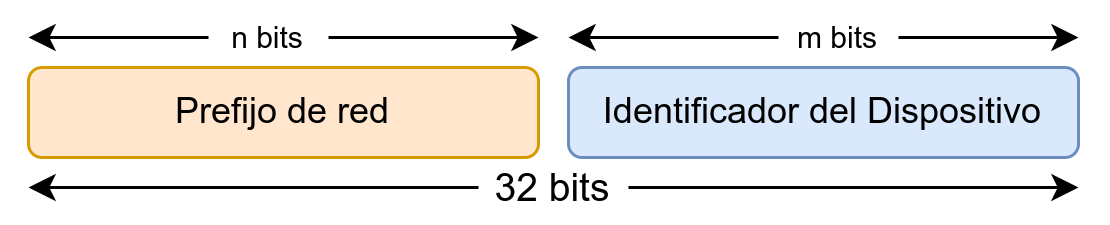
\includegraphics[width=0.8\linewidth]{mascara_de_red.png}
\end{center}

Dependiendo del número de bits que sea “n”, el número “m” variará a la par hasta que ambos sumen los 32 bits que debe de tener una dirección IP. Aquí es donde entra en juego la \textbf{máscara de red}.

La máscara de red es un número binario de 32 bits que nos permitirá conocer qué número es “n” y “m” en una dirección IP, para así obtener el prefijo de la red y conocer cuántos dispositivos puede llegar a existir en la red.

Al igual que la IP, \textbf{una máscara de red son 32 bits} que contendrán a la izquierda “n” unos y a la derecha “m” ceros.

\errorbox{
    \begin{center}
        \textbf{En la máscara de red a la izquierda irán los \texttt{1} y a la derecha los \texttt{0}.}

{\large \textbf{¡NUNCA SE MEZCLAN!}}
    \end{center}
}

Por ejemplo:
\begin{itemize}
    \item \textbf{IP decimal}:\hspace{22pt} \texttt{192.168.1.100}
    \item \textbf{IP binario}:\hspace{25pt} \texttt{11000000101010000000000101100100}
    \item \textbf{Máscara de red}: \texttt{11111111111111110000000000000000}
\end{itemize}

Si contamos el número de unos que tenemos en el lado izquierdo de la máscara de red veremos que tenemos 16, por lo que los primeros 16 bits de la IP serán los que nos digan a qué red pertenece esa IP. En este caso, y para favorecer el visionado, realizamos una separación de los bits:

\begin{itemize}
    \item \textbf{IP binario}:\hspace{25pt} \texttt{11000000\space\space10101000\space\space00000001\space\space01100100}
    \item \textbf{Máscara de red}: \texttt{11111111\space\space11111111\space\space00000000\space\space00000000}
\end{itemize}

Con esto obtenemos:
\begin{itemize}
    \item \textbf{Prefijo de la red}: \texttt{192.168}
    \item \textbf{Identificador del dispositivo:} \texttt{1.100}
\end{itemize}

Si observamos, la máscara de red, al ser 32 bits, también se puede escribir en formato decimal, aplicando al igual que antes, la creación de 4 grupos de 8 bits. En el ejemplo anterior \textbf{la máscara sería: \texttt{255.255.0.0}} .

Existe un tercer método para escribir la máscara de red:  “\textbf{/n}”, donde “\textbf{n}” es un número indicando el número de \textbf{unos} (y por tanto, los bits que identifican el prefijo de la red) que tiene la máscara de red. En nuestro caso, la máscara también se puede escribir como \textbf{/16}, ya que es el número de unos que tiene nuestra máscara.

\section{Nombre de la red, broadcast y dispositivos}

De una máscara y una IP podemos obtener más información. Para conocer el \textbf{número de posibles IPs que puede llegar a haber en esa red} tendremos que realizar el cálculo de $2^{m}$, donde “m” es el número de ceros que tiene la máscara.

En nuestro ejemplo es $2^{16} = 65536$ posibles IPs. \textbf{De estas IPs existen dos IPs especiales}:

\begin{itemize}
    \item \textbf{Nombre de la red}: El nombre de la red sirve para identificar y diferenciar las distintas redes que pueden llegar a existir.

    Es muy importante nombrarlas de manera correcta ya que nos dará la información necesaria para conocer el prefijo de la red y el número posible de dispositivos que puede haber.

    Para crear el nombre de la red lo haremos usando el prefijo de la red y el resto de bits ponerlos a 0. En nuestro ejemplo:

    \begin{center}
        \textbf{\texttt{11000000  10101000  00000000  00000000 = 192.168.0.0}}
    \end{center}

    \textbf{Al nombre de la red siempre se le debe añadir la máscara}, por lo que quedaría:  \texttt{\textbf{192.168.0.0 /16}}

    \errorbox{\textbf{Si no se pone la máscara de red, podría ser una IP suelta de cualquier red.}}

    \item \textbf{Broadcast}: Sirve para poder mandar un mensaje a todos los dispositivos de la red. Para formar esta dirección usamos el prefijo de la red y el resto de bits ponerlos a 1, por lo que en nuestro ejemplo quedaría:

    \begin{center}
        \textbf{\texttt{11000000  10101000  11111111  11111111 = 192.168.255.255}}
    \end{center}
\end{itemize}

Teniendo esto en cuenta, al total de posibles IPs de una red tendremos que restarle 2 para darnos el número total de dispositivos que podremos tener en una red:


\infobox{
\begin{center}
\textbf{Para saber el número de posibles IPs de una red: }

        {\Large $2^{m} - 2$}

\textbf{siendo “m” el número de “\texttt{0}” de la máscara}
\end{center}
}

En nuestro ejemplo vemos que “m” es 16 (porque en la máscara tenemos 16 ceros), y sabemos que tenemos 2 IPs especiales (\textbf{el nombre de la red} y \textbf{el broadcast}) que tendremos que restar para tener el número total de dispositivos (tablets, ordenadores, móviles conectados) que podrá llegar a tener esa red:  $2^{16} - 2 = 65534$ posibles dispositivos. El rango de estos dispositivos será desde la IP \texttt{\textbf{192.168.1.1}} hasta \texttt{\textbf{192.168.255.254}}.


\section{Bloques de IPs reservadas}
Dentro de todas las posibles IPs y redes que podemos llegar a crear, existen unos bloque que están \href{https://en.wikipedia.org/wiki/Reserved_IP_addresses}{reservados} por unas razones u otras:

\begin{itemize}
    \item \textbf{Redes públicas}: son todas las IPs que no entran en los siguientes bloques, y por tanto, son las utilizadas públicamente en Internet.

    \item \textbf{Redes privadas}: Son redes que sólo pueden existir en el ámbito privado y no se podrá configurar de cara internet.

    \item \textbf{Reservado}: Existen varios bloques que están reservados por diversas razones, de los cuales veremos los ejemplos más característicos.
\end{itemize}

Es importante conocer los bloques reservados para no cometer errores a la hora de crear redes. El listado completo se puede encontrar en la \href{https://es.wikipedia.org/wiki/IPv4#Direcciones_de_uso_especial}{Wikipedia}.


\subsection{Bloque reservado: 127.0.0.0 /8}

La primera dirección de este bloque, 127.0.0.1, es el utilizado como bucle local (o \textbf{loobpack}). Este conjunto de IPs hacen referencia al propio equipo en el que nos encontramos y se suelen utilizar para hacer pruebas locales.


\subsection{Redes privadas}

Una red privada es una red de computadoras que usa el espacio de direcciones IP especificadas más adelante. A los equipos o terminales se les puede asignar direcciones de este espacio cuando deban comunicarse con otros terminales dentro de la red interna/privada.

Los nombre de las redes privadas son:

\begin{itemize}
    \item \textbf{\texttt{10.0.0.0 /8}}
    \item \textbf{\texttt{172.16.0.0 /12}}
    \item \textbf{\texttt{192.168.0.0 /16}}
\end{itemize}

Estas redes privadas no son siempre utilizadas con su máxima máscara posible, ya que en la mayoría de los casos se estarían desperdiciando IPs.

El utilizar en nuestra red privada un rango que no sea uno de estos tres signfica que estamos yendo en contra de las reglas establecidas por la ICANN.

\subsection{Reservado para despliegues Carrier Grade NAT}

En abril de 2012, el IANA asignó el rango \textbf{100.64.0.0/10} para uso en escenarios de \href{https://es.wikipedia.org/wiki/Carrier_Grade_NAT}{Carrier Grade NAT} en el \href{https://www.rfc-editor.org/rfc/rfc6598}{RFC 6598}.

Este bloque de direcciones no debe ser usado en redes privadas o en la Internet pública: ha sido pensado para operaciones de uso interno en redes de teleoperadores. El tamaño del bloque de direcciones (aproximadamente 4 millones de direcciones, $2^{22}$) ha sido seleccionado para ser suficientemente grande para acomodar todos los dispositivos de acceso de un solo operador en un punto de presencia en una red de área metropolitana como la de Tokio (Fuente: \href{https://es.wikipedia.org/wiki/Carrier_Grade_NAT}{Wikipedia}).

\subsection{Bloque reservado para el futuro}
Existe el bloque completo \textbf{\texttt{240.0.0.0 /8}} cuyas IPs están reservadas para pruebas y para el futuro. Es conocido como la “clase E”.


\subsection{Otros bloques}
Como ya se ha comentado, en la \href{https://en.wikipedia.org/wiki/Reserved_IP_addresses}{Wikipedia} se pueden encontrar todos los bloques reservados que no son públicos y la razón por las que han sido reservados.


\section{Clases de IP}
Durante el inicio de la expansión de internet y la creación de redes se crearon clases que nos indican el número de subredes que deberían existir, la máscara y más información que \textbf{hoy en día se considera obsoleta}.

\begin{itemize}
    \item \textbf{Clase A}: se asigna el primer octeto para identificar la red, reservando los tres últimos octetos (24 bits) para que sean asignados a los hosts, de modo que la cantidad máxima de hosts es $2^{24} - 2$ . El bit más significativo (el de más a la izquierda) empieza por 0.

    \item \textbf{Clase B}: se asignan los dos primeros octetos para identificar la red, reservando los dos octetos finales (16 bits) para que sean asignados a los hosts. Los primeros bits más significativos son 10:

    \item \textbf{Clase C}: se asignan los tres primeros octetos para identificar la red, reservando el octeto final (8 bits) para que sea asignado a los hosts, de modo que la cantidad máxima de hosts por cada red es $2^{8} - 2$ . Los primeros bits más significativos son 110
\end{itemize}

\section{Configurar IPv4}

Una vez sabemos cómo funciona IPv4, es el momento de aplicarlo en el sistema operativo en el que nos encontremos.

\subsection{IPv4 en Windows}

Por defecto, la configuración de red en Windows solicita una dirección IP de manera automática cuando el cable está conectado en el interfaz de red.

Para conocer la configuración actual de la red podemos utilizar el comando \commandbox{ipconfig} desde el terminal de windows. Si le pasamos el parámetro “/all” ( \commandbox{ipconfig /all} ), el resultado del comando nos dará más información, como es la configuración del DNS, la dirección física (MAC), ...

\begin{center}
    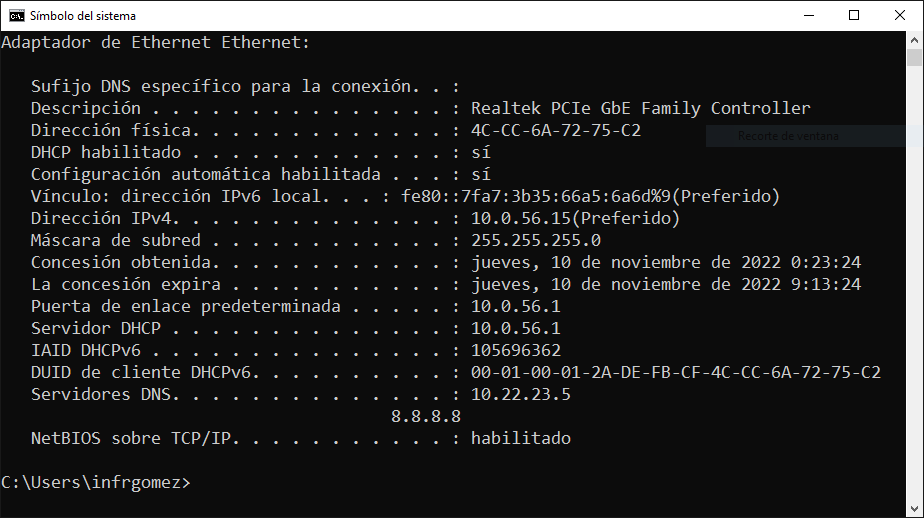
\includegraphics[width=0.8\linewidth]{ipconfig.png}
\end{center}


Si queremos realizar la modificación de la red, podremos hacer uso del icono de red que está al lado de la hora. Para ver toda la configuración, podemos ir al “Panel de Control → Redes e Internet → \textbf{Configuración de Red e Internet}”. Elegimos “Protocolo de Internet versión 4”, le damos a “Propiedades” y podremos realizar la configuración siguiente:


\begin{center}
    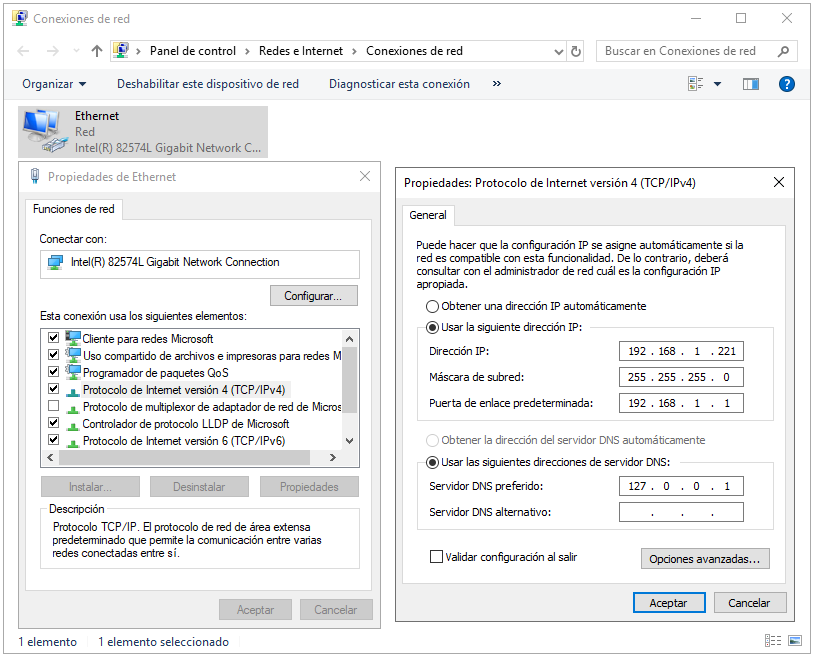
\includegraphics[width=0.7\linewidth]{cambiar_ip_windows.png}
\end{center}


En la imagen se puede ver la configuración realizadA:
\begin{itemize}
    \item \textbf{Dirección IP}: La dirección IP que queremos que tenga el equipo.
    \item \textbf{Máscara de subred}: La máscara de red a la que pertenece la IP que hemos configurado.
    \item \textbf{Puerta de enlace predeterminada}: Para que el equipo tenga conexión con otras redes, debemos indicar qué IP tiene el \textbf{\textit{gatway}}.
\end{itemize}

Aparte, podemos realizar la configuración del servidor DNS primario y secundario.